\subsubsection{lead}
We design a lead controller with siso tool box.
$$
C(s) = \dfrac{16.231(s + 2.51)}{s + 6.963}
$$
\begin{itemize}
	\item all figures from siso toolbox
	\begin{figure}[H]
		\caption{All figures from siso toolbox}
		\centering
		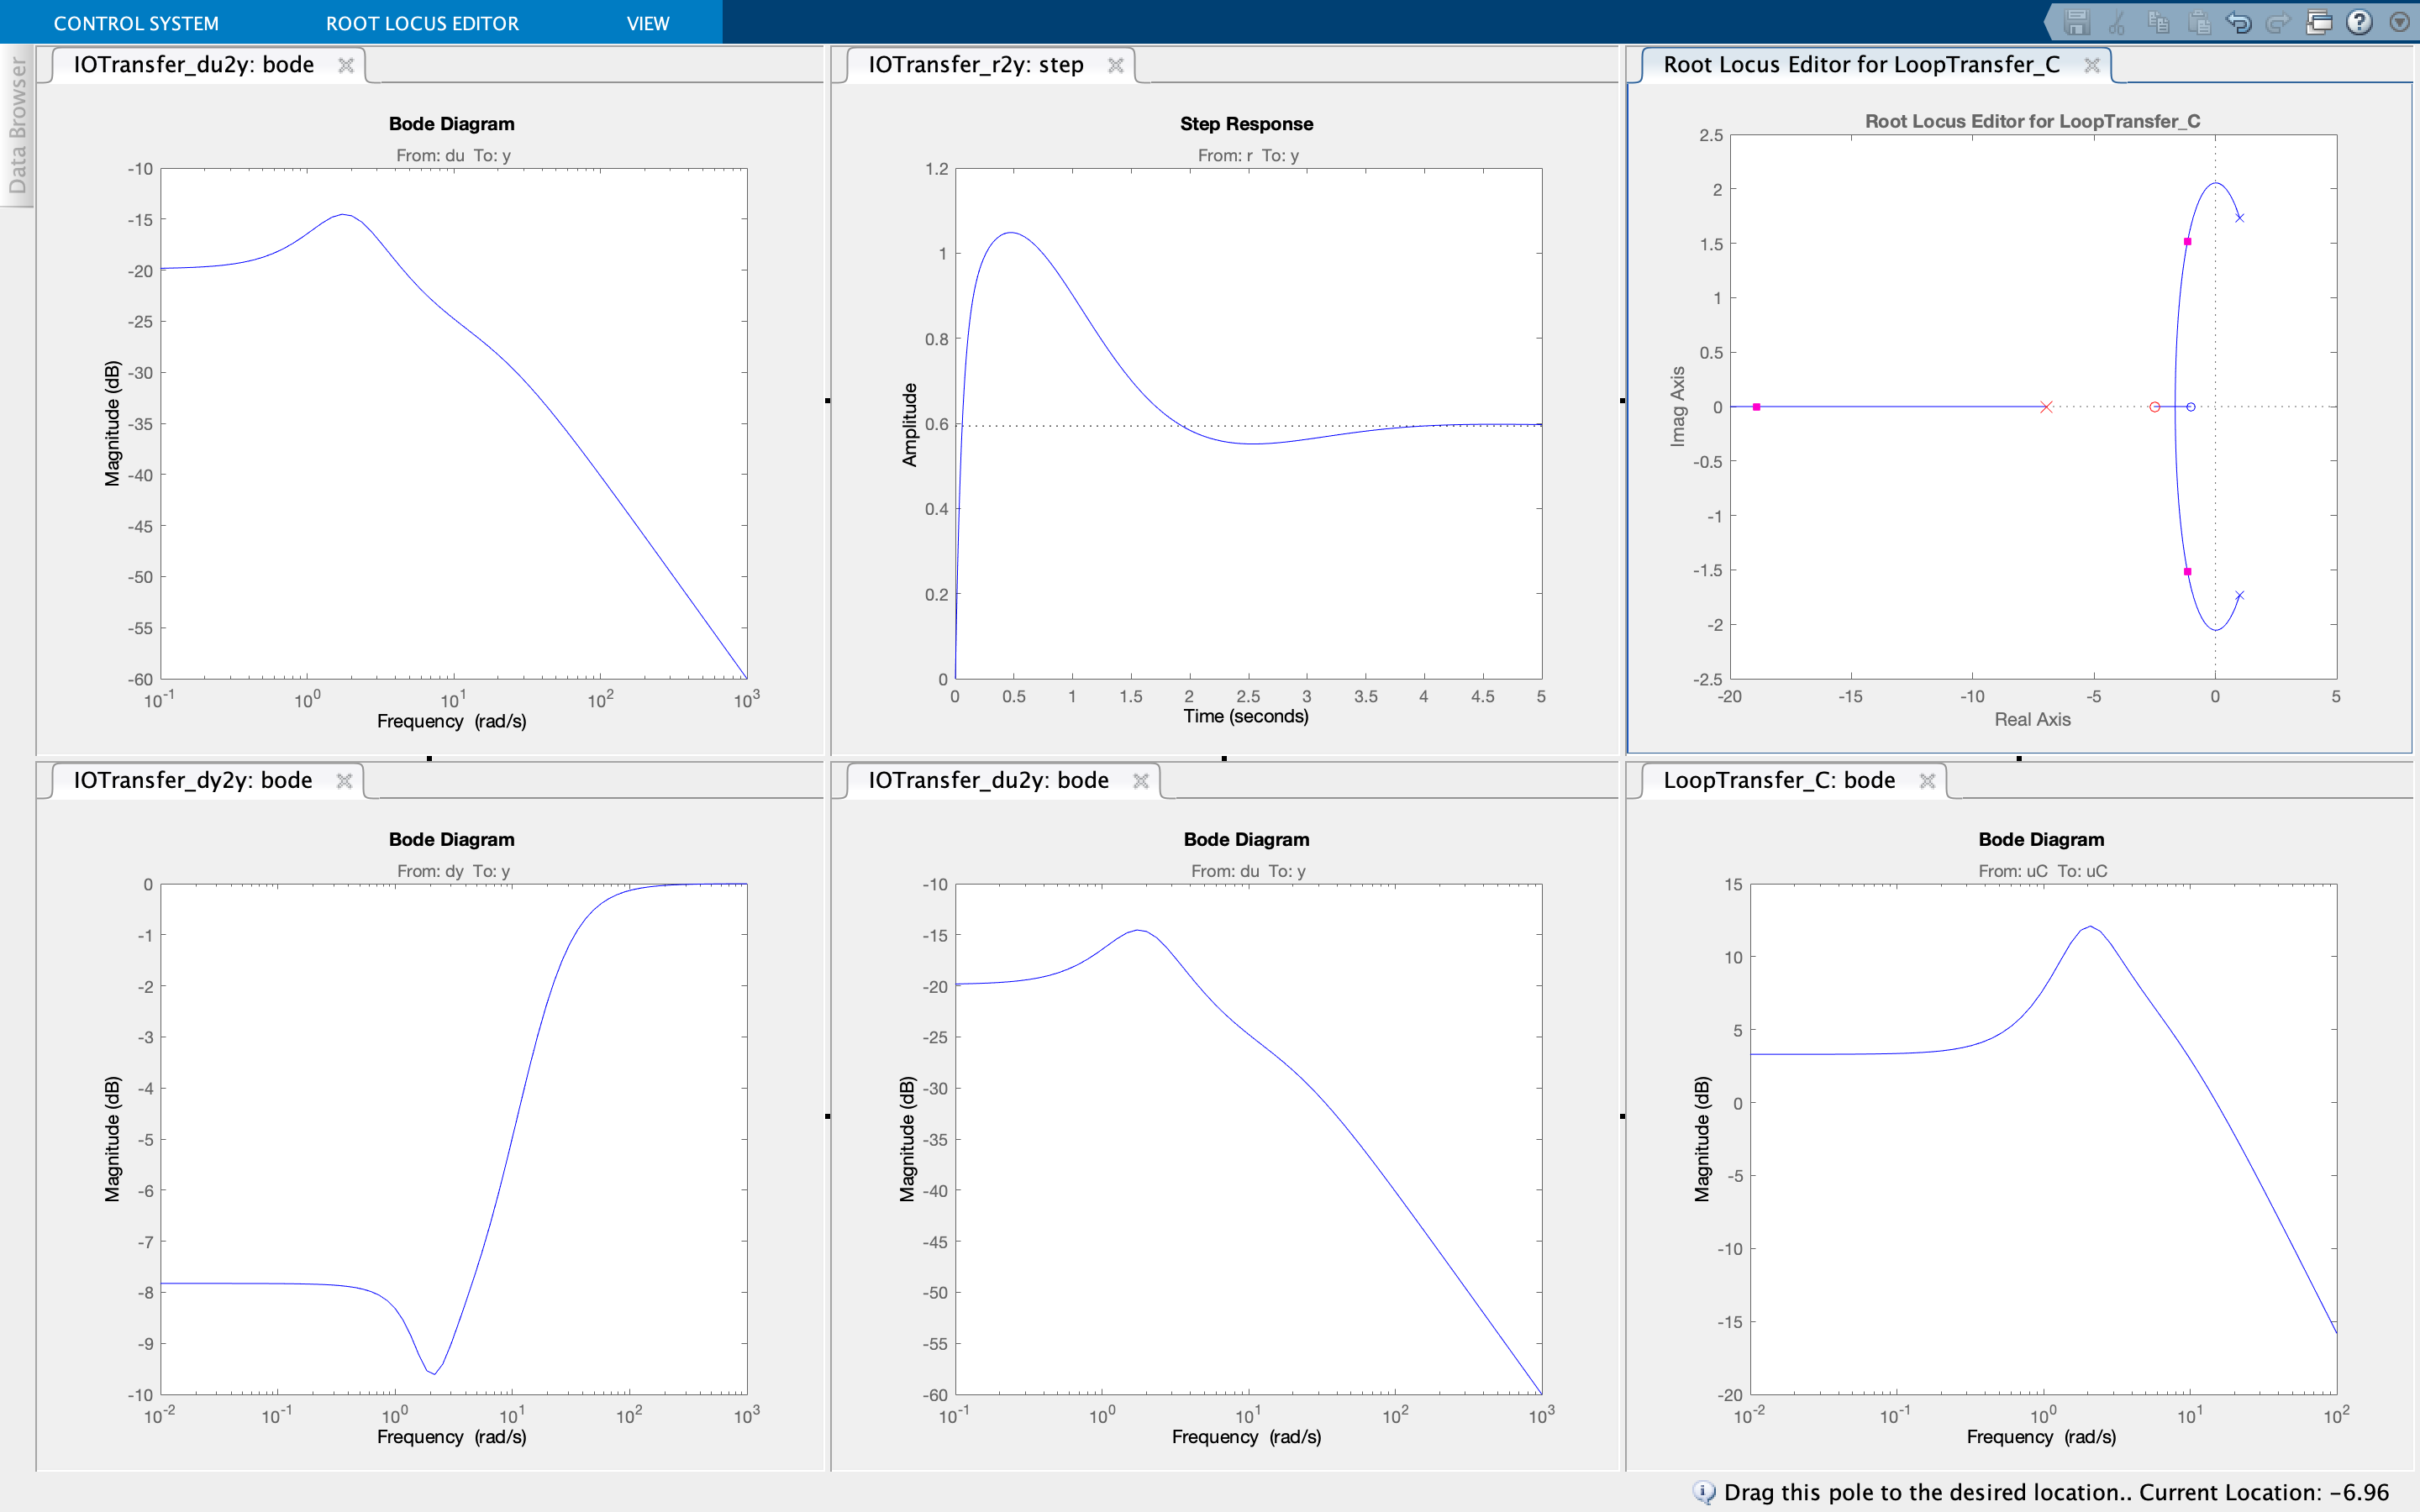
\includegraphics[width=16cm]{../Figure/Q1/Q1_b/lead/siso_all.png}
	\end{figure}
	\newpage
	\item root locus with lead controller
	\begin{figure}[H]
		\caption{root locus}
		\centering
		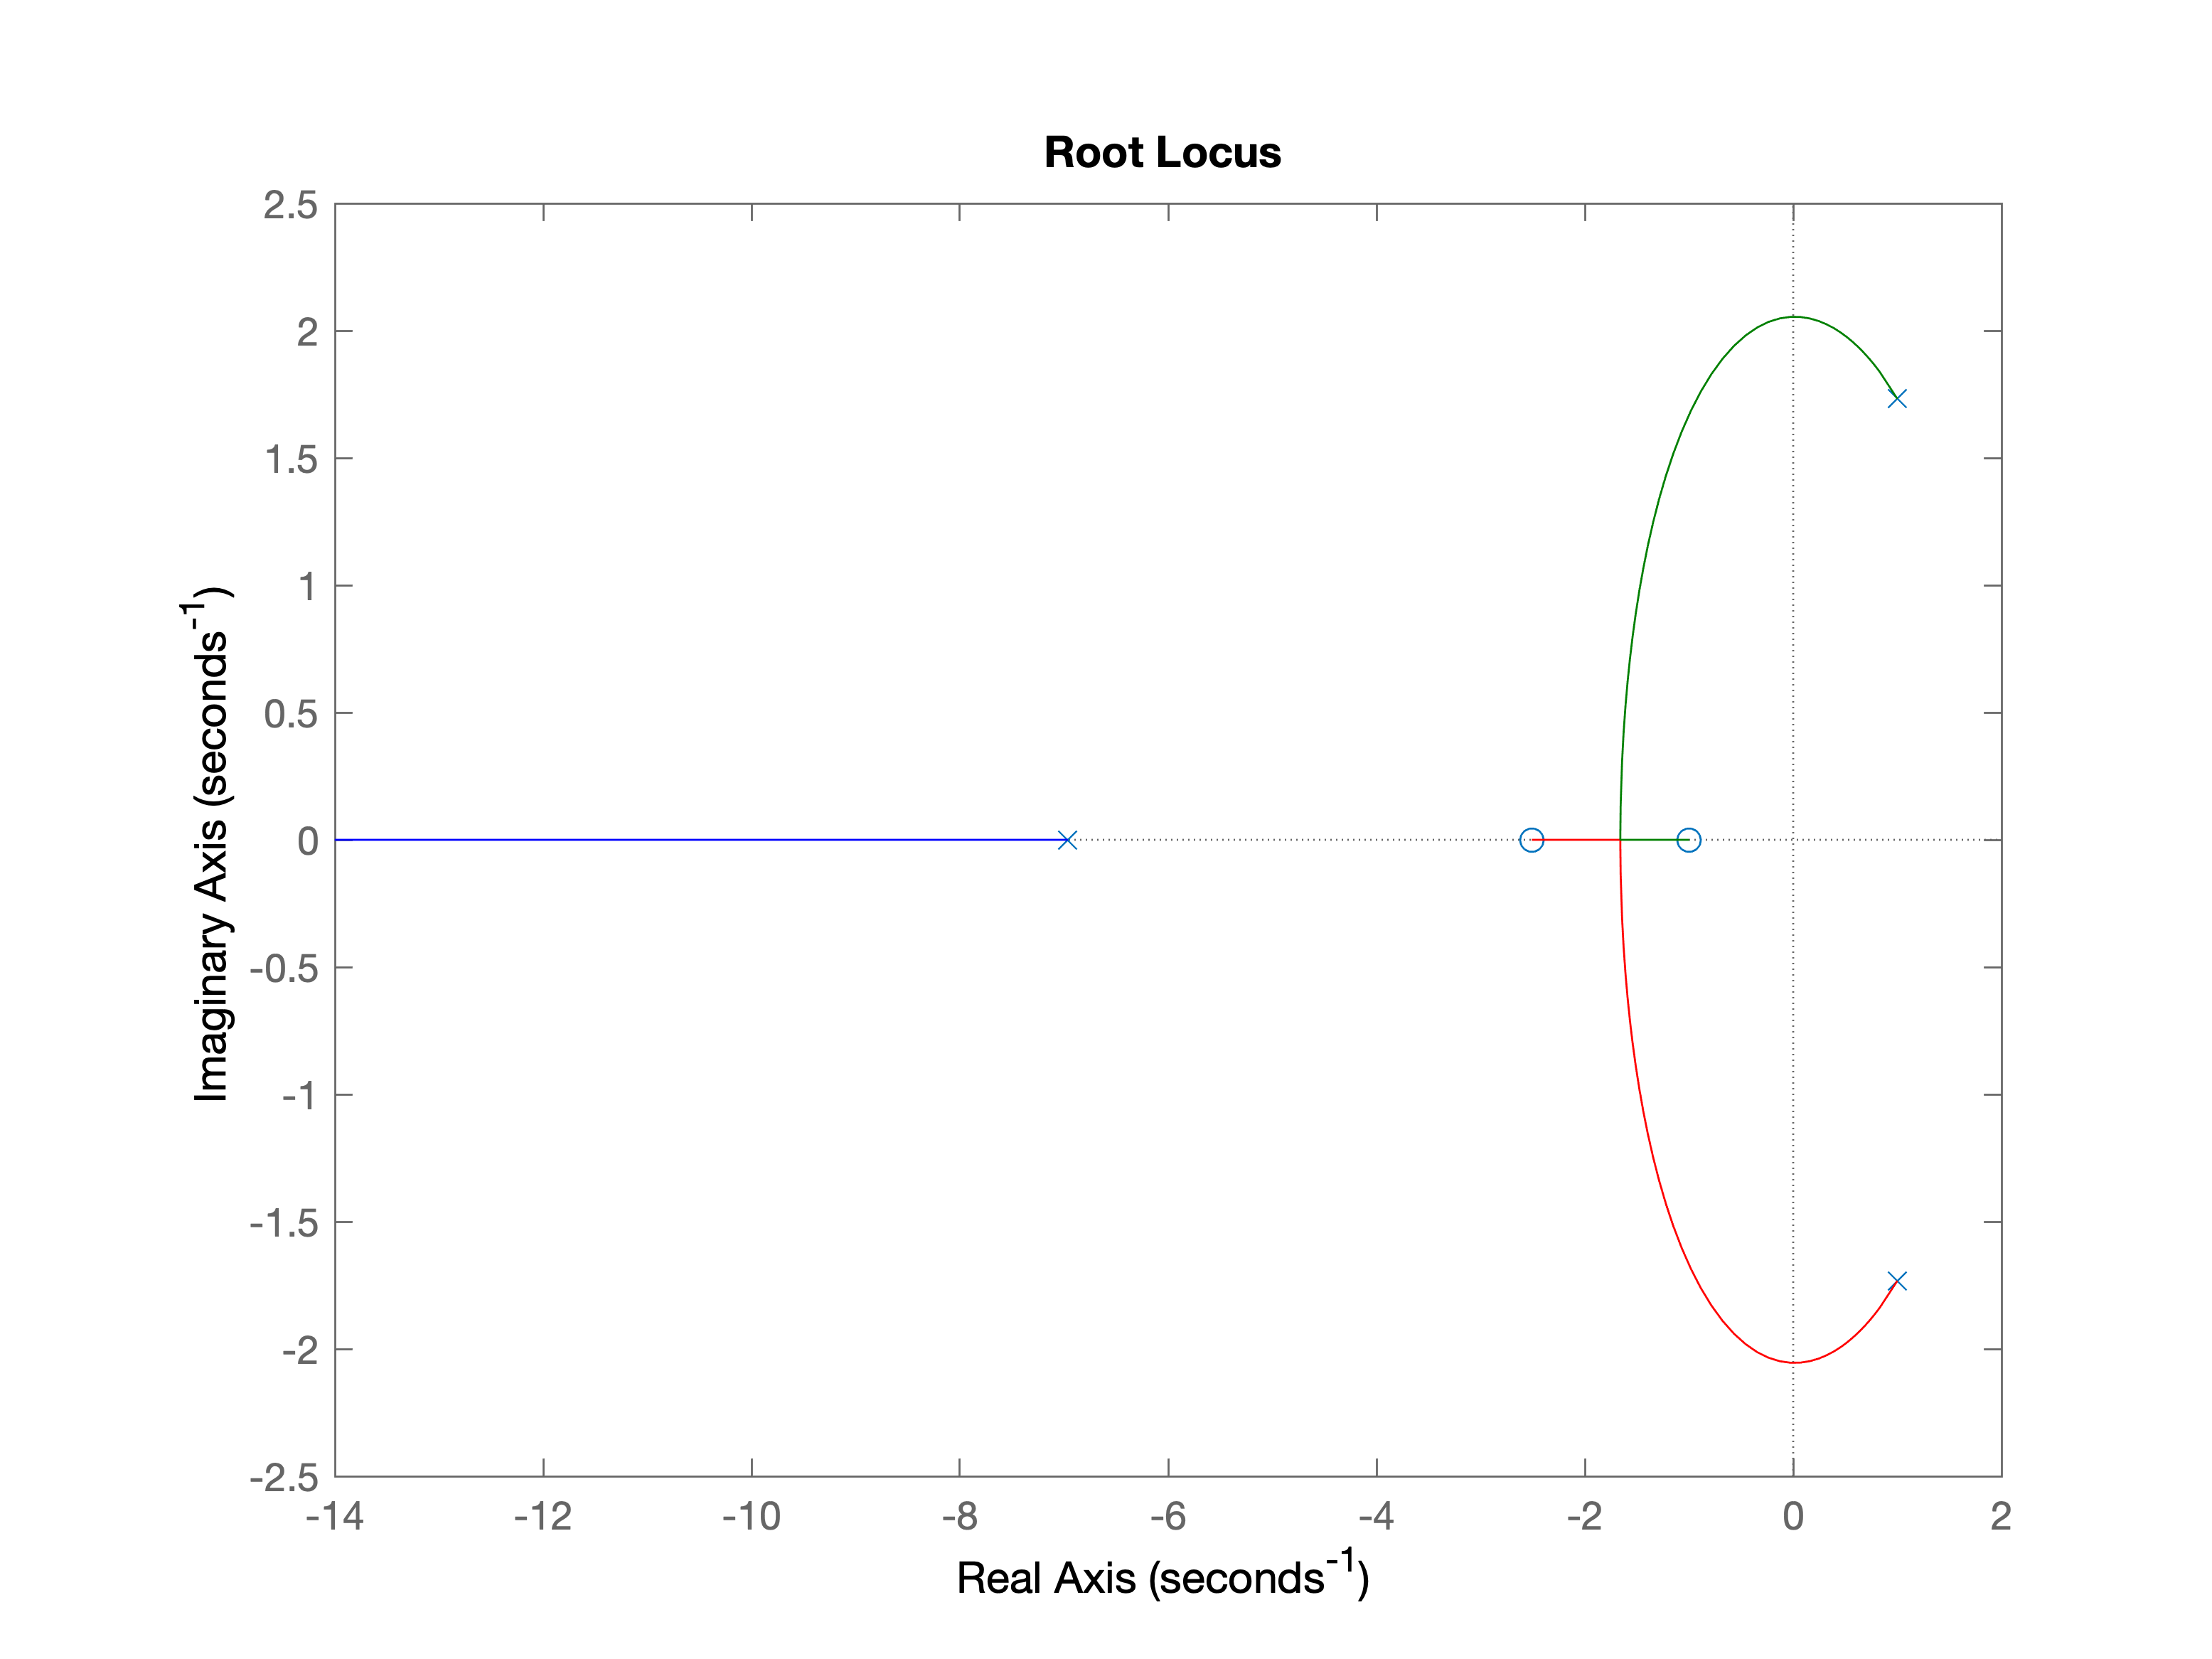
\includegraphics[width=12cm]{../Figure/Q1/Q1_b/lead/rlocus.png}
	\end{figure}
	\item step response for closeloop system with lead controller
	\begin{figure}[H]
		\caption{step response for closeloop system}
		\centering
		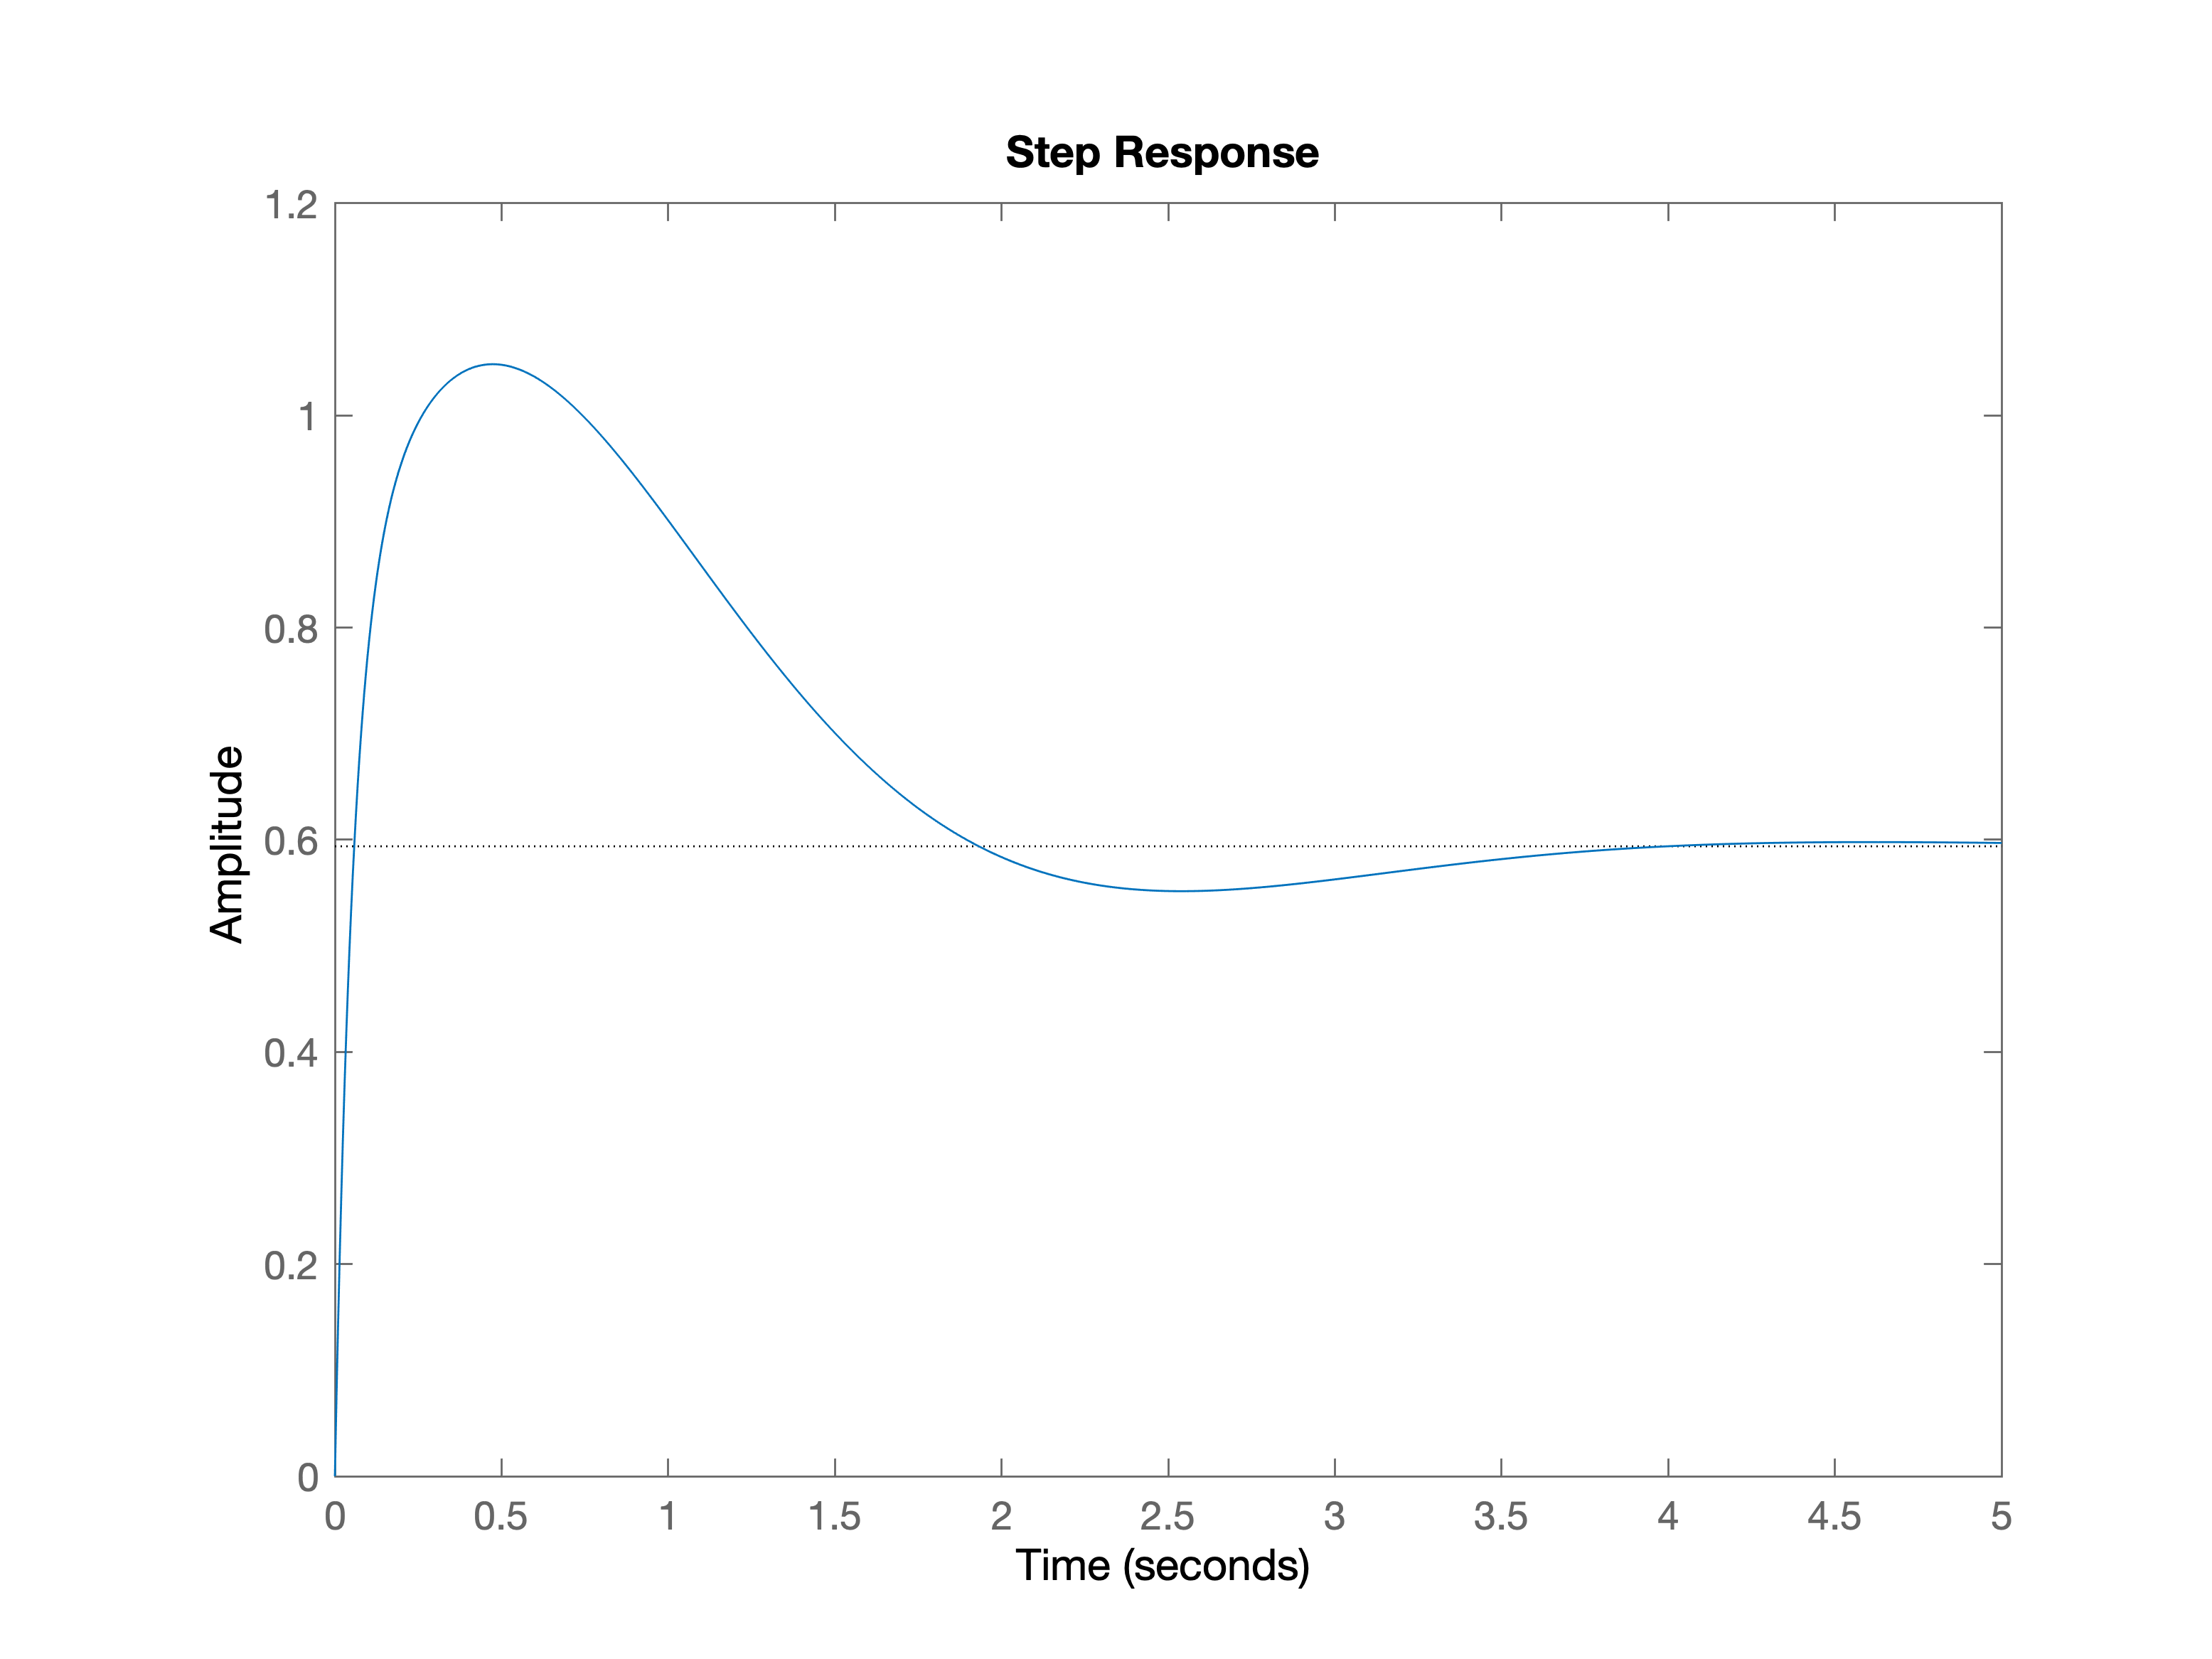
\includegraphics[width=12cm]{../Figure/Q1/Q1_b/lead/feedback_step.png}
	\end{figure}
	\item closeloop bode (magnitude) with lead controller
	\begin{figure}[H]
		\caption{closeloop bode (magnitude)}
		\centering
		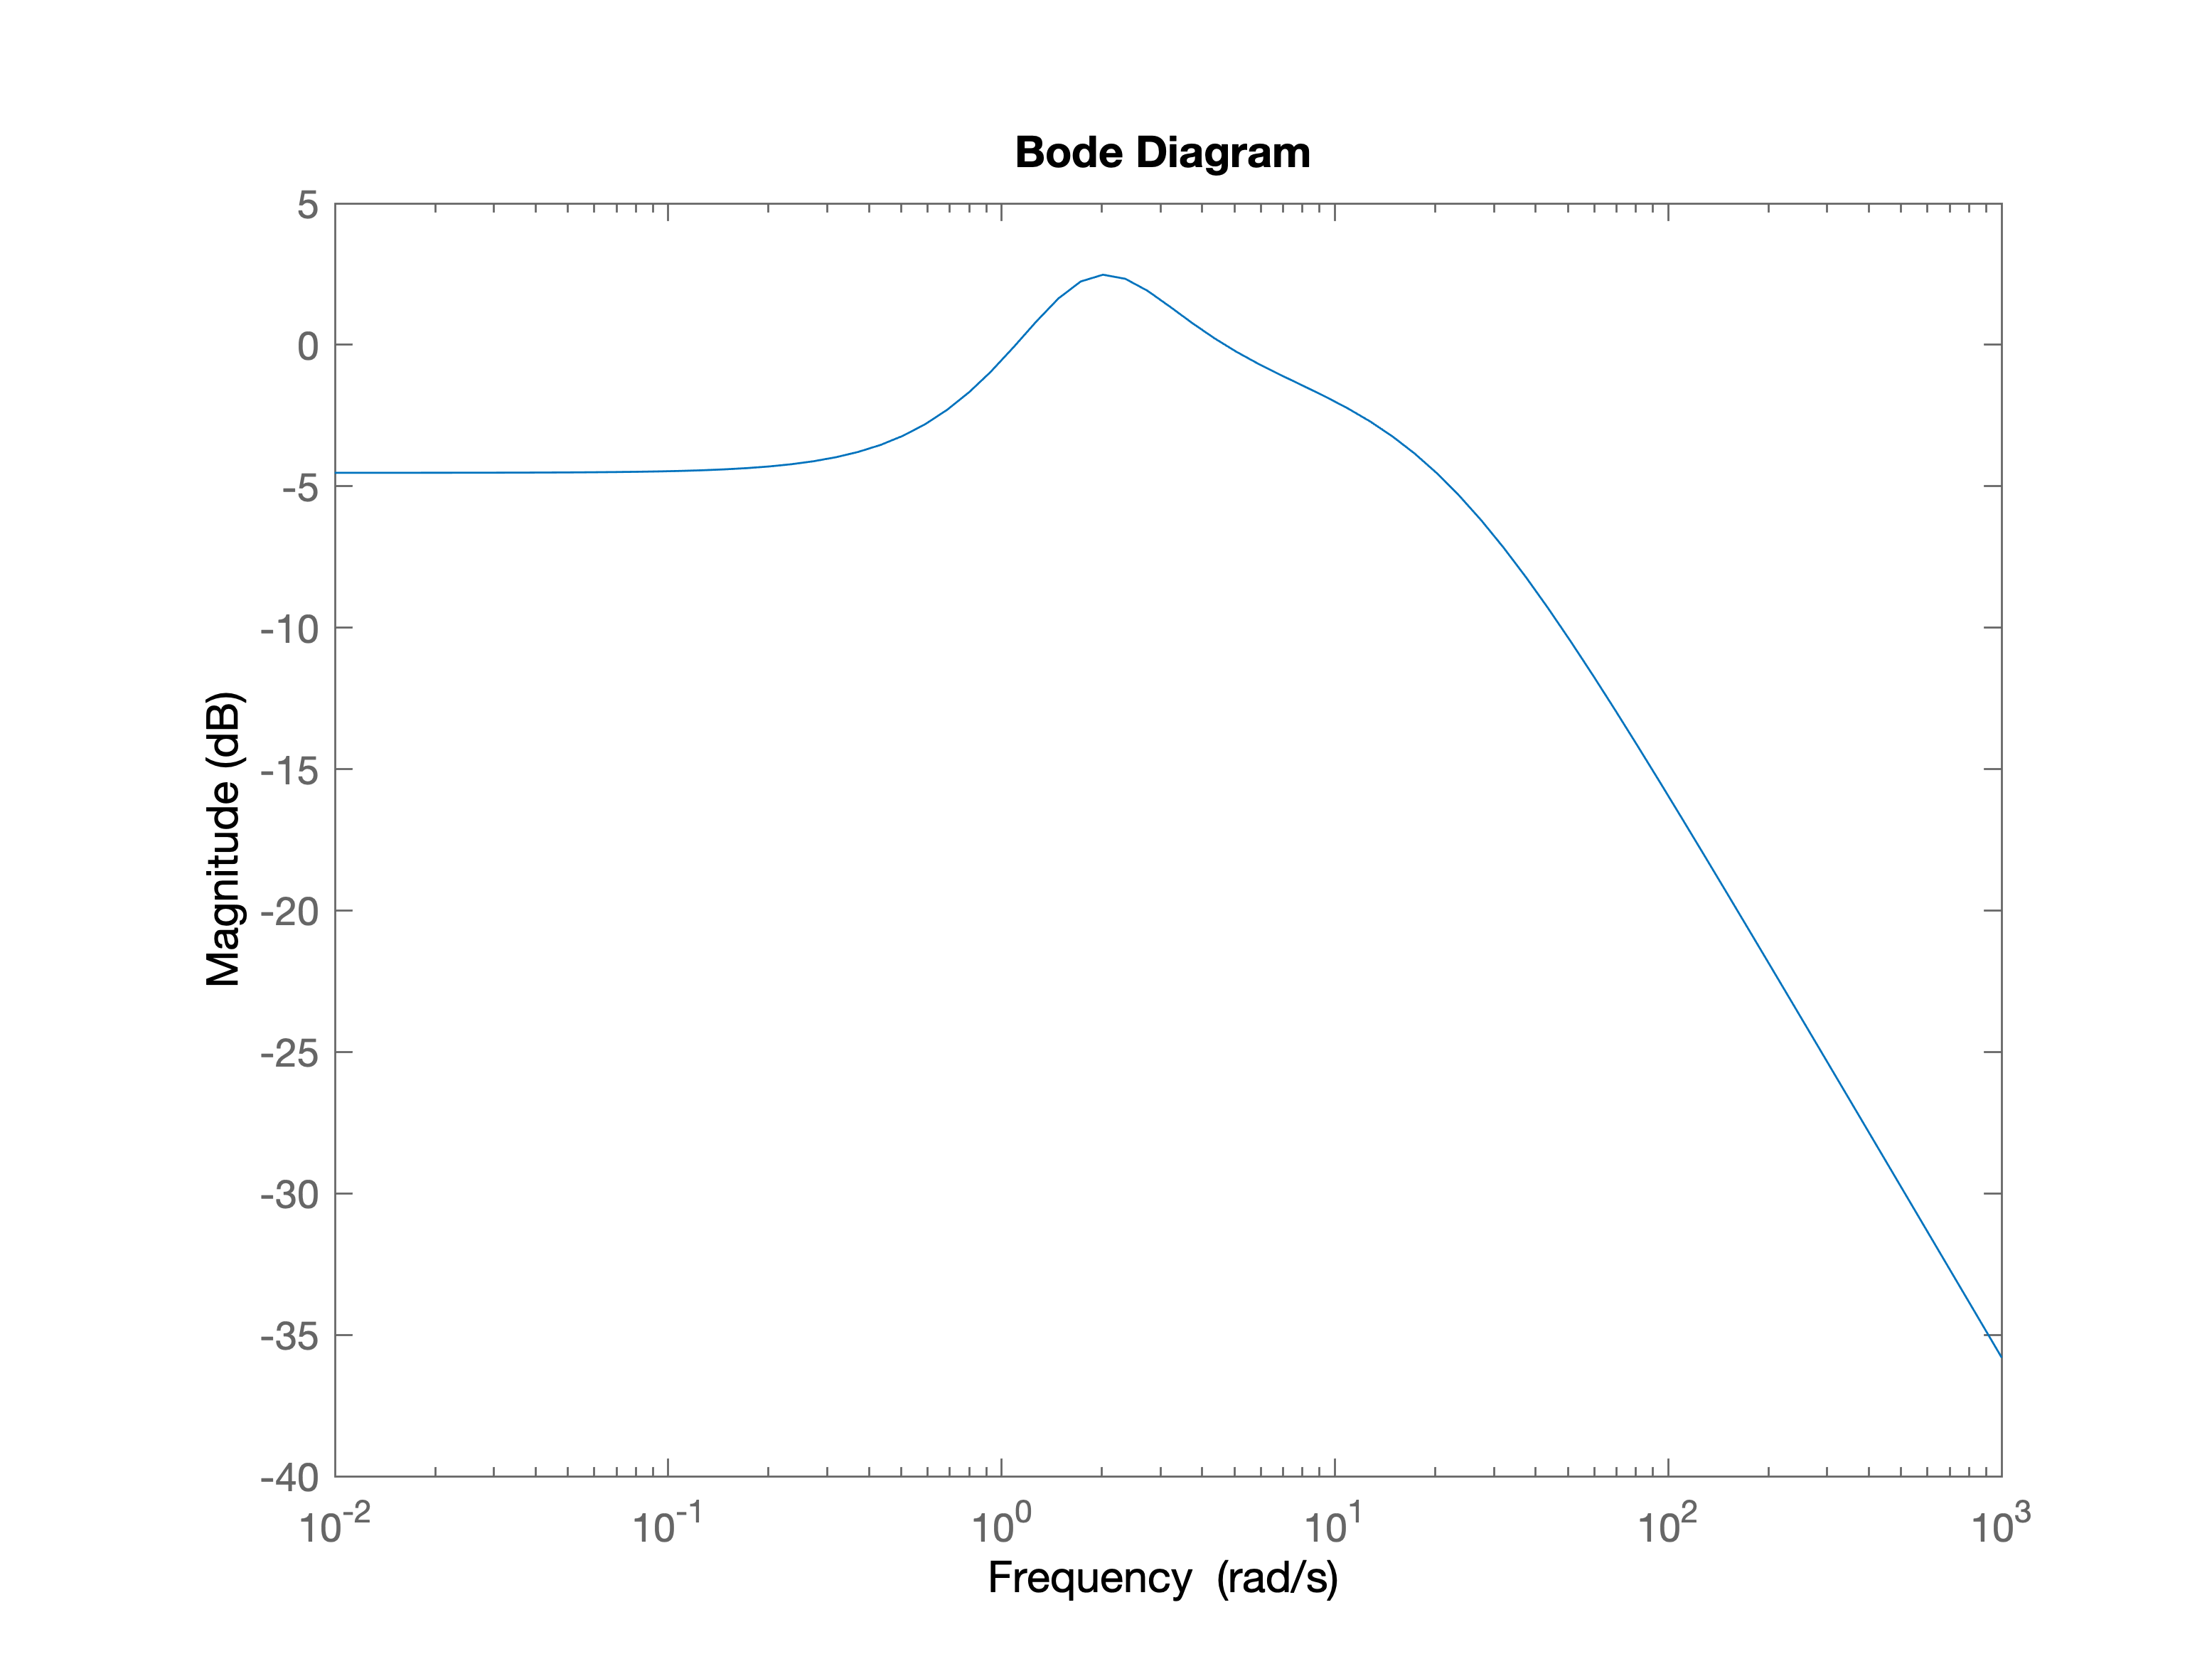
\includegraphics[width=12cm]{../Figure/Q1/Q1_b/lead/feedback_bode.png}
	\end{figure}
	\item openloop bode (magnitude) with lead controller
	\begin{figure}[H]
		\caption{openloop bode (magnitude)}
		\centering
		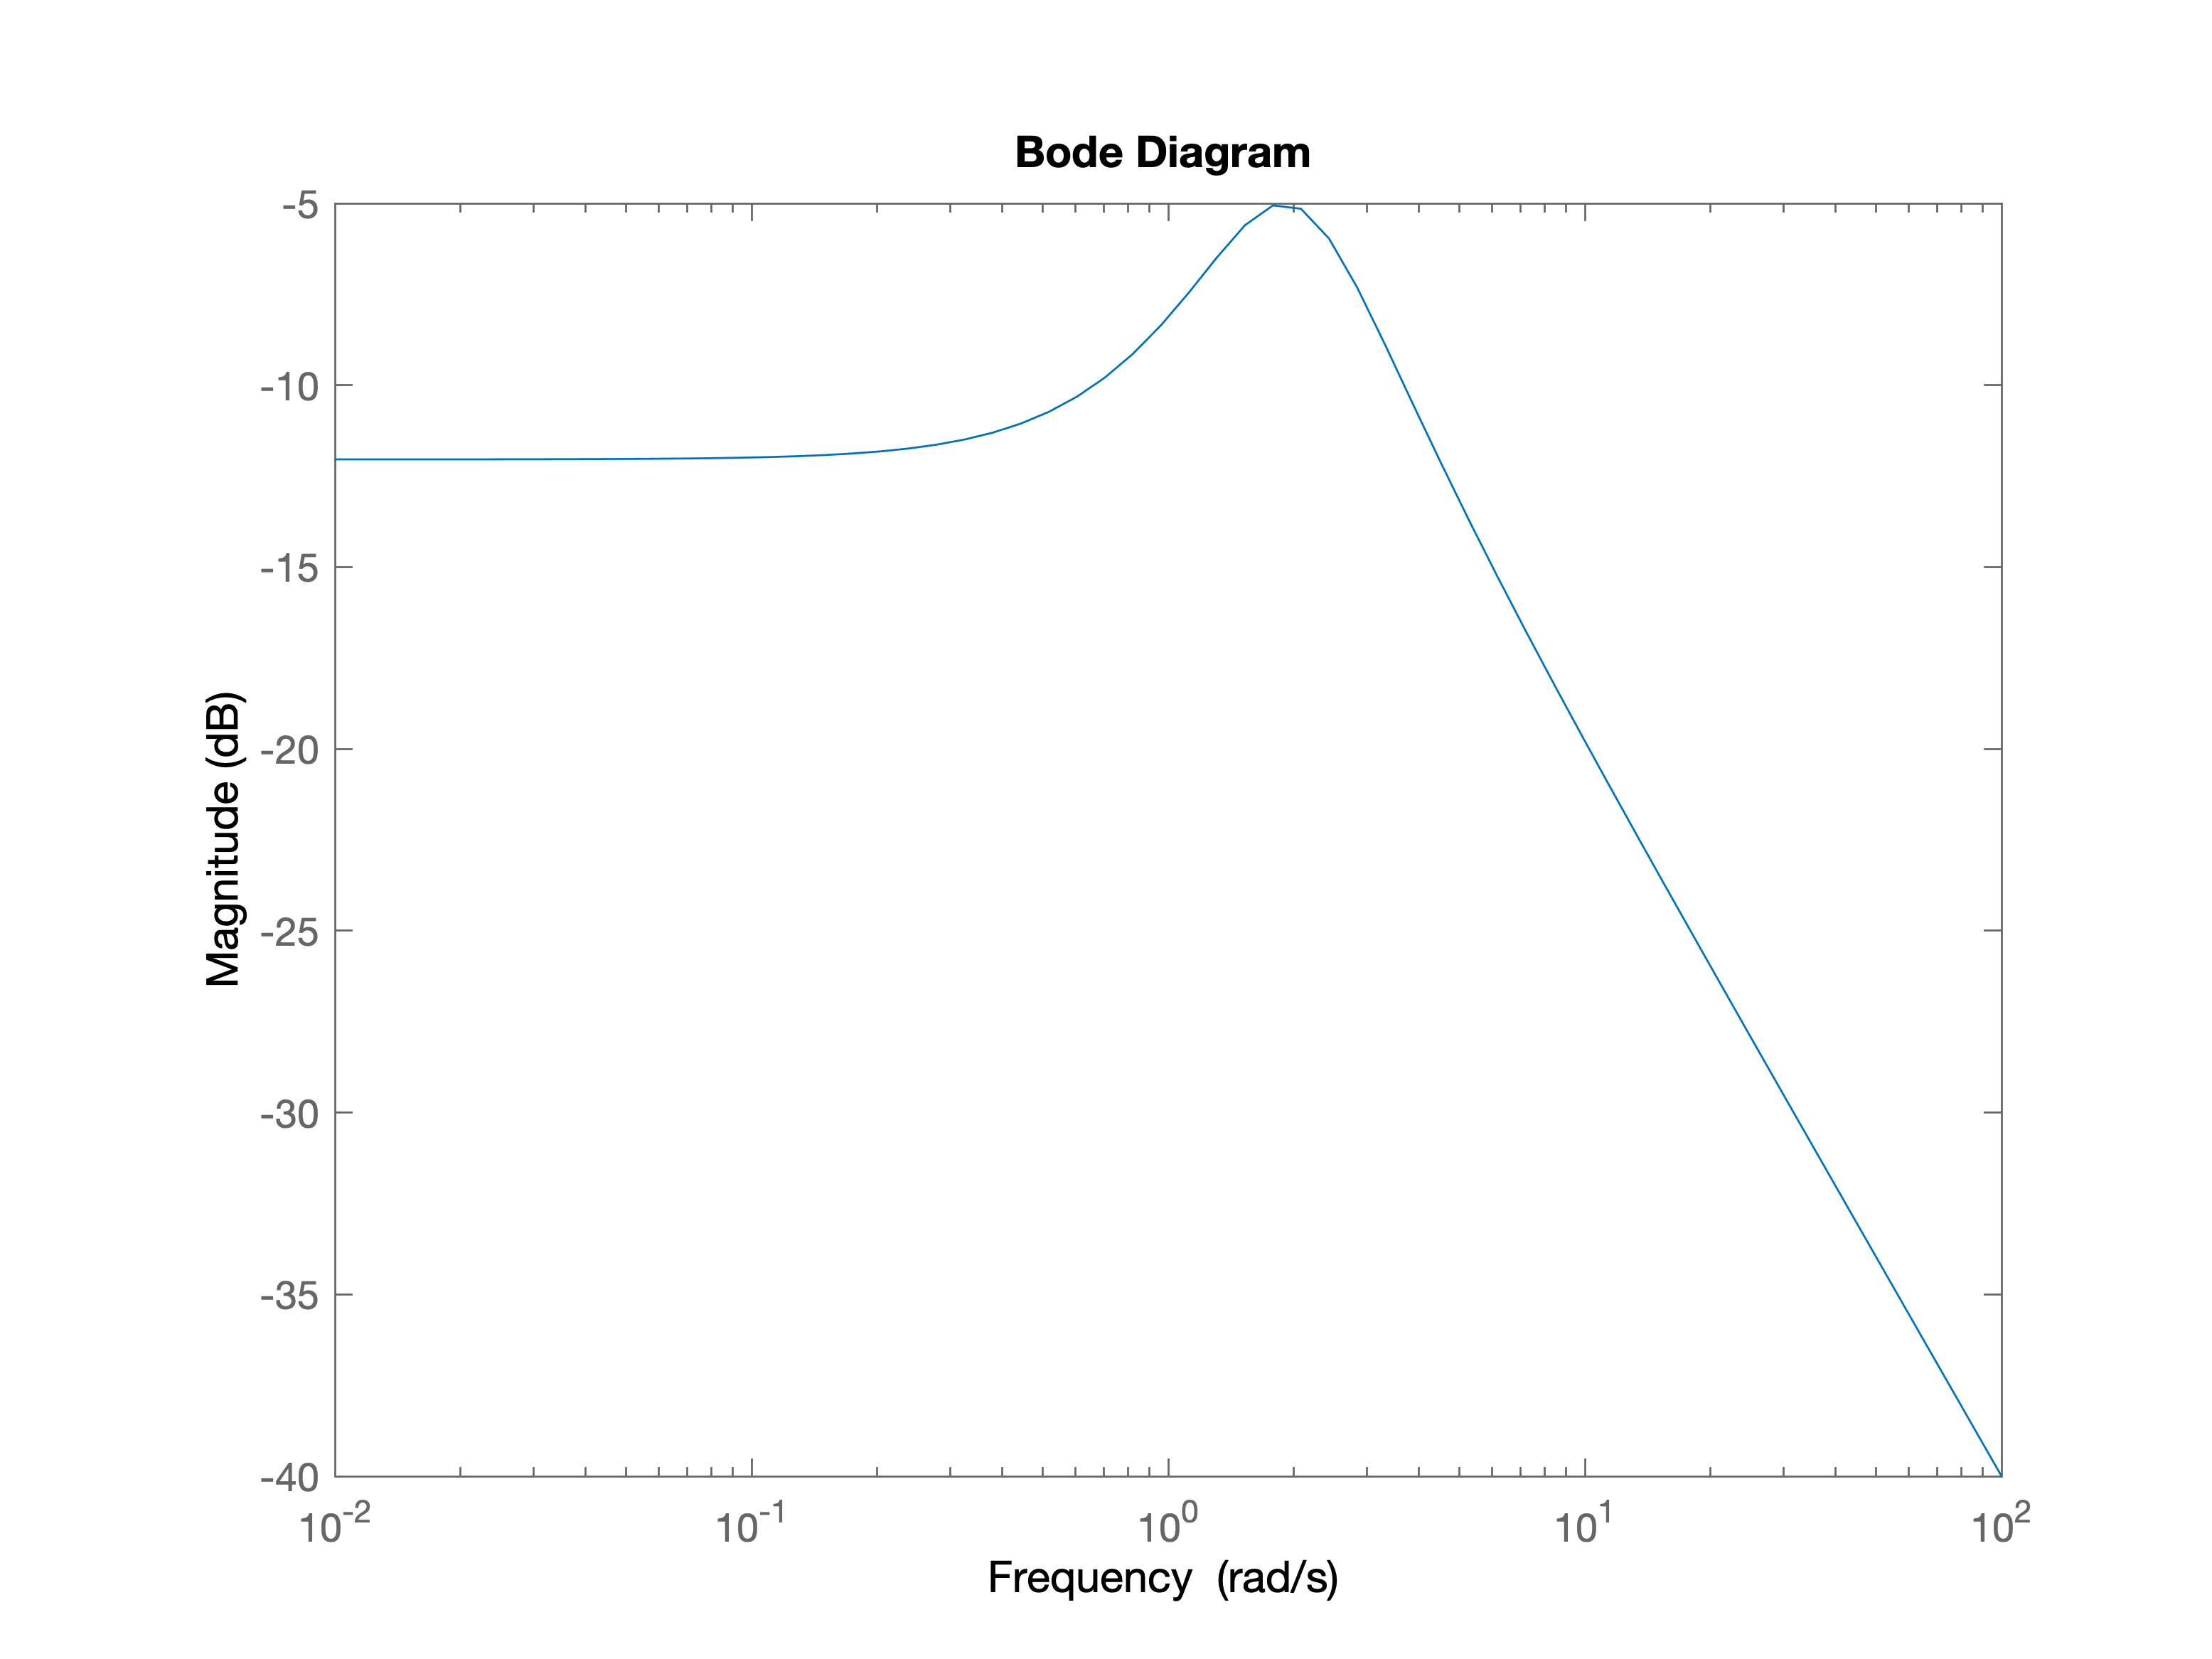
\includegraphics[width=12cm]{../Figure/Q1/Q1_b/lead/openloop_bode.png}
	\end{figure}
	\item sensitivity function with lead controller
	\begin{figure}[H]
		\caption{sensitivity function}
		\centering
		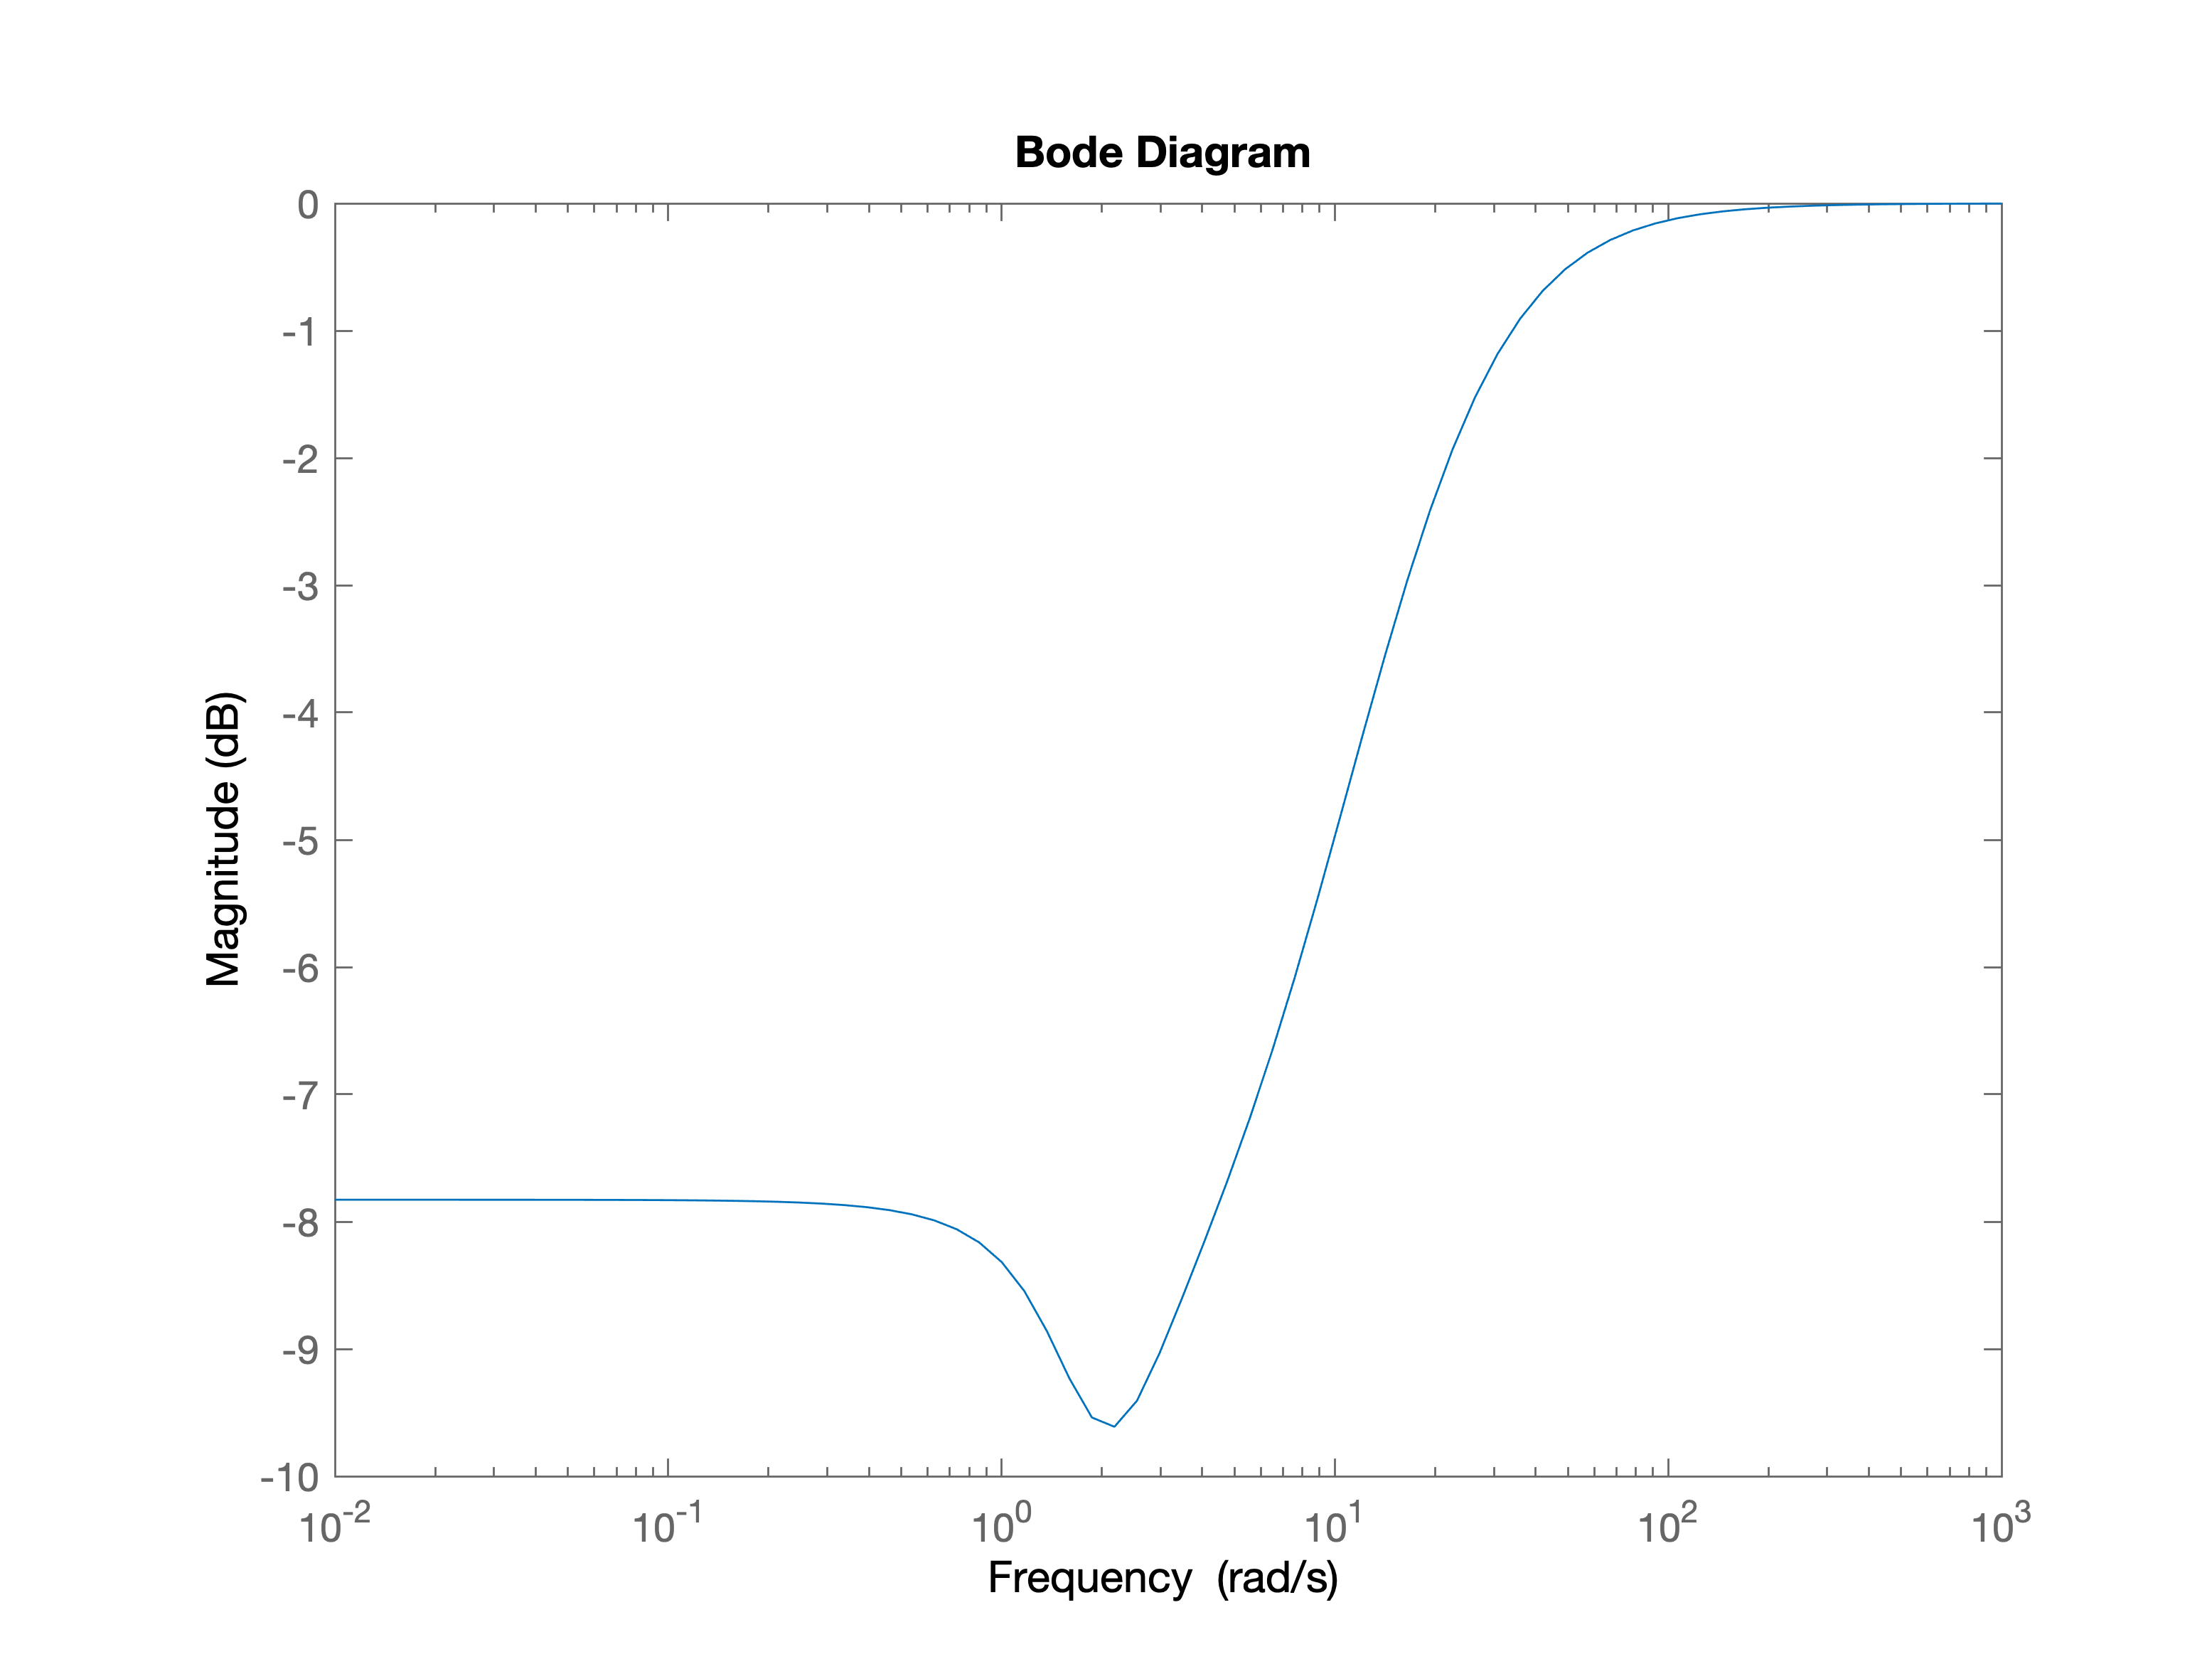
\includegraphics[width=12cm]{../Figure/Q1/Q1_b/lead/s_bode.png}
	\end{figure}
	\item complementary sensitivity function with lead controller
	\begin{figure}[H]
		\caption{complementary sensitivity function}
		\centering
		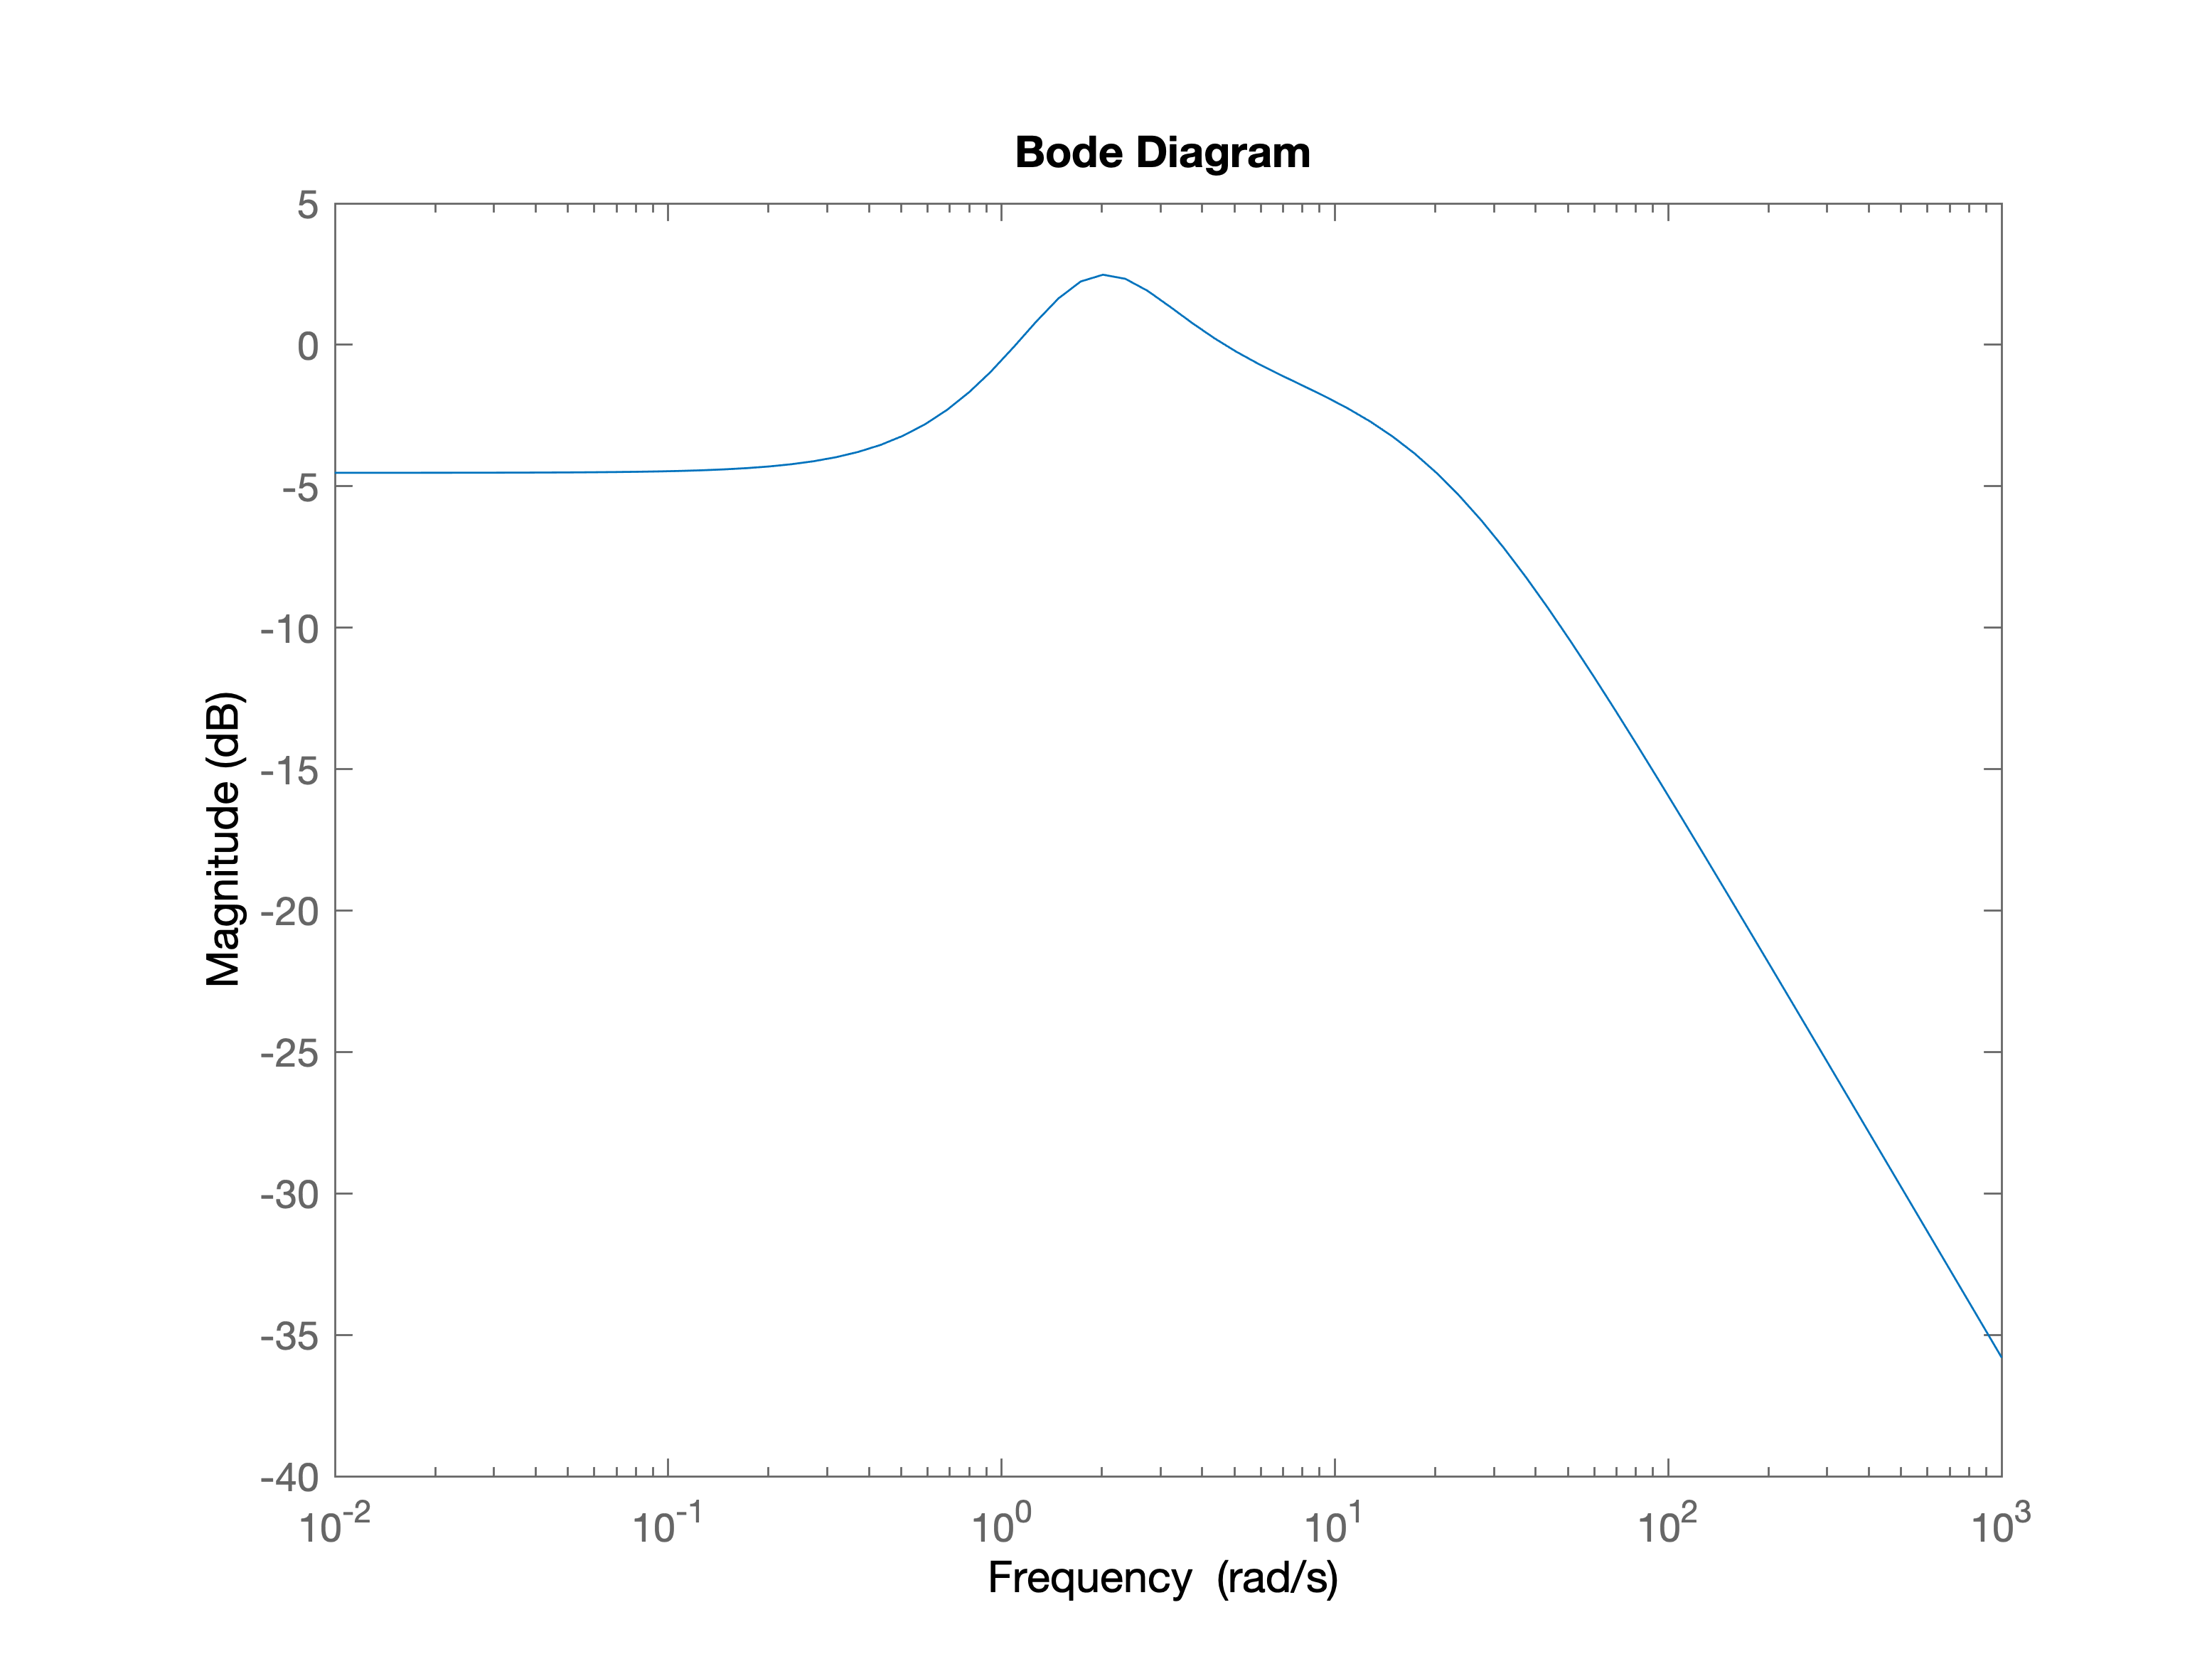
\includegraphics[width=12cm]{../Figure/Q1/Q1_b/lead/t_bode.png}
	\end{figure}
\end{itemize}
System is stable with controller and have a noise cancelation for frequancy after $100_{rad/{\sec}}$ and it have effect on system about $-20_{dB}$. System have very good disturbance rejection about $1_{rad/{\sec}}$ and have a good disturbance rejection about $10_{rad/{\sec}}$ and disturbance have effect on system about $-5_{dB}$. 

In this question we don't know what is plant and actuator and how noise or disturbance effect on system and about what frequancy so we assume that noise is about more than $100_{rad/{\sec}}$ and disturbance is about $10_{rad/{\sec}}$ and$-5_{dB}$ is a low effect and system work well.

No. System have staedy state error. we could increase gain in controller but it needed very high gaib controller and no actuator can do this so we can't make staedy state error zero with this requirements.